\documentclass[10pt,twocolumn,letterpaper]{article}

\usepackage{cvpr}
\usepackage{times}
\usepackage{epsfig}
\usepackage{graphicx}
\usepackage{amsmath}
\usepackage{amssymb}
\usepackage{subfig}
\graphicspath{ {images/} }
% Include other packages here, before hyperref.

% If you comment hyperref and then uncomment it, you should delete
% egpaper.aux before re-running latex.  (Or just hit 'q' on the first latex
% run, let it finish, and you should be clear).
\usepackage[breaklinks=true,bookmarks=false]{hyperref}

\cvprfinalcopy % *** Uncomment this line for the final submission

\begin{document}
	
	%%%%%%%%% TITLE
	\title{Music Genre Classification}
	
	\author{Mark Gameng\\
		Illinois Institute of Technology\\
		{\tt\small mgameng1@hawk.iit.edu}
	}
	
	\maketitle
	
	\begin{abstract} % DONE
		In this paper, I propose a deep learning framework for utilizing dual feature spectrogram inputs instead of the usual single input done by many others. This framework, named Dual CNN + Classical, consists of two feature inputs that is fed to two separately trained CNN models and then concatenated to a classical algorithm classifier. Experimental results using GTZAN and Extended Ballroom dataset show that this type of framework yields similar or better accuracies than models only utilizing one feature input. For Extended Ballroom, a Dual CNN + SVM model using STFT and MFCC input achieves 92.4\% accuracy. For GTZAN, a Dual CNN + KNN model using STFT and Melspectrogram input achieves 95.8\% accuracy. 
	\end{abstract}

	\section{Introduction} % DONE
	
	Music, throughout the years, have been skyrocketing in terms of music generation and have also resulted in new styles/genres of music. Music platforms in general are producing thousands of new songs each day, with Spotify having listed over 50 million songs and over 40 thousand new songs are added every day. Years ago, the genre of songs were classified manually by people with musical knowledge. With the amount of music generation in our current era, it is imperative that music genre classification be automated through musical analysis and machine learning. Automated music genre classification will allow platforms like Spotify, Pandora, Soundcloud to better serve its customers by having a more accurate search and recommender systems. Because of this, the interest in the field of Music Information Retrieval (MIR) has been increasing ever since. Specifically, one popular topic that has garnered countless studies in MIR is music genre classification.
	
	With machine learning, computer scientists have been trying to tackle the automation of music genre classification and recently, have achieved pretty good results. A model can only learn to classify genre of music by looking at the features of it. Thus, feature extraction is one of the most important parts in music genre classification. In the past, feature extractions were done manually but currently, automatic feature extraction is done through machine learning. With just a spectrogram or any image that is able to accurately represent music, machine learning algorithms, more specifically Convolutional Neural Networks (CNN), are able to extract features and classify the genre at a very high accuracy.
	
	Previous works have tried many ways to tackle music genre classification from logistic regression up to neural networks. Notably, most high accuracy models use neural networks either on its own, or combined with another algorithm, and they all achieve in the 80\% range or higher. A few of the best models that achieved the highest accuracy is done using a method called MusicRecNet + SVM~\cite{elbir2020music} and Broadcast NN~\cite{liu2020bottom} that got 97.6\% and 97.2\% respectively. Most of the published methods are trained on only one type of spectrogram such as a Short-time Fourier Transforms (STFT). While STFTs alone may be enough to achieve a good genre classification accuracy, combining models with different spectogram inputs may result in higher accuracies. This combination would be somewhat similar to the architecture proposed by Yang et al~\cite{yang2020parallel} that used a CNN and a bi-directional RNN in parallel with an input of STFT. Instead, with multiple feature spectrogram inputs, there would be multiple different CNN or RNN in parallel. Classical algorithms such as logistic regression, support vector machine will probably also increase accuracy when combined with other deep learning methods. 
	
	Interested by the problems above, I propose a framework that consists of using two different feature inputs that is fed to two separately trained CNN and concatenated to a classifier that uses a classical algorithm. I also used a selection of input lengths and various classical algorithms to further determine the best combination that would lead to a high music genre classification accuracy.
	
	\section{Related Works} % DONE
	
	Music genre classification is a widely studied area in music information retrieval. A person or a machine learning model can only learn to classify the genres of music by looking at specific features that pertains to that specific genre. As a result, feature extraction is a crucial part in music genre classification. In this regard, most high accuracy models utilize CNNs due to their ability to learn the more representative features of the music samples on their own. Other methods have also been done such as Yang et al~\cite{yang2020parallel}. using a CNN in parallel with a bidirectional recurrent neural network to extract spatial and temporal features of music. With deep learning methods, one does not need to be an expert in music to point out specific features to look at for genre classification and attain high levels of accuracy.  
	
	Thus, most recent published models in music genre classification consists of CNNs and spectrograms as an input. Some of the top models have achieved 97.6\%, 97.2\%, and 92.5\% accuracy which are named MusicRecNet + SVM~\cite{elbir2020music}, Broadcast NN~\cite{liu2020bottom} , and CNN + 2-layer RNN~\cite{yang2020parallel} respectively. These models either used STFT or melspectrograms as an input, similar to most other high performing models. Other than using spectrograms as a feature input, others have also added additional inputs such as lyrics and cover image of music. Oramas et al~\cite{oramas2017multi} proposed a multimodial approach that outperforms a single modality approach with the aggregation of audio, lyrics, and cover image achieving the best results. In the field of music genre classification, there are still improvements to be had and many approaches that have not been thought of and utilized to further increase the already high accuracy attained by recent models.
	
	\section{Data} % DONE
	
	GTZAN~\cite{tzanetakis2002musical} dataset is widely used for music genre classification. It is a public dataset that consists of 1,000 audio clips that are 30 seconds each and are equally classified to 10 different genres. The 10 genres are blues, classical, country, disco, hiphop, jazz, metal, pop, reggae, and rock.
	
	Extended Ballroom~\cite{marchand2016extended} is another dataset that is gaining popularity which is an improved version of the well-known Ballroom dataset. This dataset contains 4,180 tracks that are 30 seconds each and are classified to 13 different ballroom genres. The 13 genres are chacha, jive, quickstep, rumba, samba, tango, viennesewaltz, waltz, foxtrot, pasodoble, salsa, slowwaltz, and wcswing, Out of the 13, 9 genres have 252 to 529 tracks each while the last 4 genres only have about 50 tracks each.
	
	\subsection{Processing} % DONE
	
	GTZAN and Extended Ballroom only have 1,000 and 4,180 tracks with 10 and 13 genres respectively. GTZAN has equally distributed tracks while Extended Ballroom does not. Thus, 4 ballroom genres- Pasodoble, Salsa, Slow Waltz, Wcswing - were removed for having less than 100 tracks. This resulted in 1,000 tracks for GTZAN and 3,992 tracks for Extended Ballroom. The tracks were 30 seconds each and thus are able to be split up into shorter segments. This would allow for more data to train and test on. I opted to splitting the tracks by 10, 8, 5, 4, 2, 1 segments subsequently, which would result in more samples while also being able to test how much the time affects accuracy for music genre classification. This resulted in at max, 10,000 samples for GTZAN and 39,920 samples for Extended Ballroom. Compared to the original dataset, this amount of samples is much better and would result in the models less likely to overfit.
	
	The following features were extracted using the Python Librosa package: Short-time Fourier Transform (STFT), Mel-frequency Cepstral Coefficients (MFCC), and Melspectrogram, which are also shown in Figure~\ref{fig:features}. Currently, STFT is the most widely used in the top accuracy models done by others. STFT simply represents a signals amplitude as it varies over time at different frequencies. MFCC are coefficients that make up an Mel-frequency spectrum (MFC) that has the frequency bands equally spaced on the mel scale which is similar to how humans perceive sounds. Somewhat similar to MFCCs, Melspectrograms are spectograms where the frequencies are converted to mel scale. Specifically, the following parameters for feature extraction were used: n\_fft is set to 2048, hop length is 1024, number of MFCCs is 13, and number of mels is 64.
	
	\begin{figure}[!htpb]
		\centering
		\subfloat[\centering STFT]{{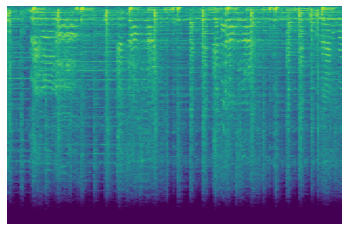
\includegraphics[width = 3.5cm]{STFT.png}}}
		\qquad
		\subfloat[\centering MFCC]{{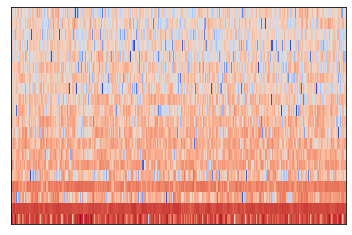
\includegraphics[width = 3.5cm]{MFCC.png}}}
		
		\subfloat[\centering Melspectrogram]{{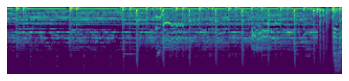
\includegraphics[width = 5cm]{MELSPECTROGRAM.png}}}
		\caption{Feature Extraction from Audio}
		\label{fig:features}
	\end{figure}
	
	\section{Methodology} % DONE
	
	Due to the low amount of samples in both GTZAN and Extended Ballroom dataset, splitting the samples into multiple segments is beneficial in terms of accuracy and generalization. Thus, the tracks were split into 10, 8, 5, 4, 2, 1 segments with no overlap which results in the samples ranging from 3 seconds to 30 seconds of audio. With a split of 10 segments for each sample, GTZAN now has 10,000 samples and Extended Ballroom with 39,920. 
	
	For model training, 20\% of samples were set aside for testing. This resulted in 80\% of the samples being used for training, in which 20\% of that is used for validation. Thus, it is a 64-16-20 split for training, validation, and testing. Aside from sample splitting, other methods were used such as early stopping, regularization, and dropouts for neural networks to avoid overfitting. A Python library for artifical neural networks, Keras, was used for building and training the CNN model. While CNN training, the best model is determined and used using the least validation loss through model checkpoints. When training using the Dual CNN + Classical architecture, hyperparameter tuning was done for the classical algorithms using GridSearchCV from the Scikit-learn Python library. The following sections further describe the methods and architectures used.
	
	\subsection{CNN} % DONE
	
	\begin{figure}[!htpb]
		\centering
		\subfloat{{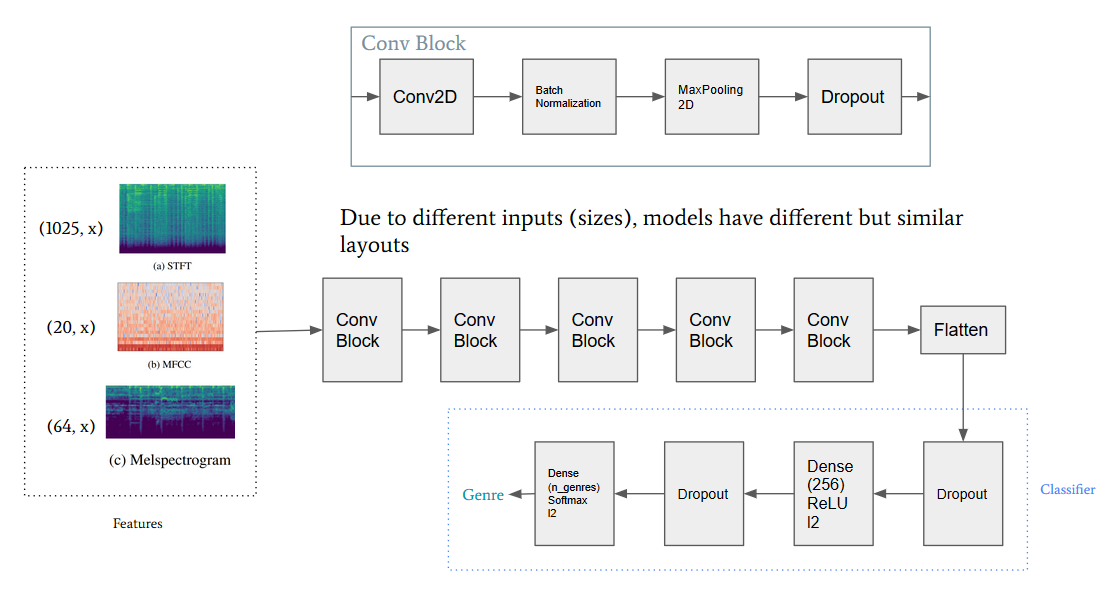
\includegraphics[width = 8cm]{CNN.png}}}
		\caption{CNN Architecture}
		\label{fig:cnn}
	\end{figure}
	
	As illustrated in Figure~\ref{fig:cnn}, the proposed CNN architecture consists of 4 to 5 convoluted blocks followed by a flatten operation and then fed to a classifier block. Due to the different shapes of the spectrograms for the input, the models for each feature vary a little from each other, however the general structure is the same. The spectograms has the shapes (1025, 64), (20, 64), (64, 64) with 10 splits for STFT, MFCC, and Melspectrogram respectively. As a result for the smaller shapes, I decided to use 4 convolutional layers for MFCC and Melspectrogram while using 5 for STFT. After each convolutional layer, batch normalization, max pooling operation, and dropout of 0.25 is done to overall reduce overfitting and extract only the most needed music features. The convolutional layers all have padding, kernel size of (3, 3), and strides of (1, 1) with rectified linear units (ReLUs) activation function. The filters for STFT are (16, 32, 64, 128, 64) and for MFCC and Melspectrogram, (32, 64, 128, 64). For the max pooling operation, pool size is (2, 2) and strides is (2, 2).
	
	After it has gone through all the convolutional layers, the output is flattened and a 0.5 dropout is once again used. The result is then fed to a dense layer of 256 neurons and a ReLU activation with l2 regularization. Afterwards, a 0.25 dropout is performed again followed by a final dense layer of \#genres neurons with softmax activation to classify the music genre.
	
	\subsection{Dual CNN + Classical} % DONE
	
	\begin{figure}[!htpb]
		\centering
		\subfloat{{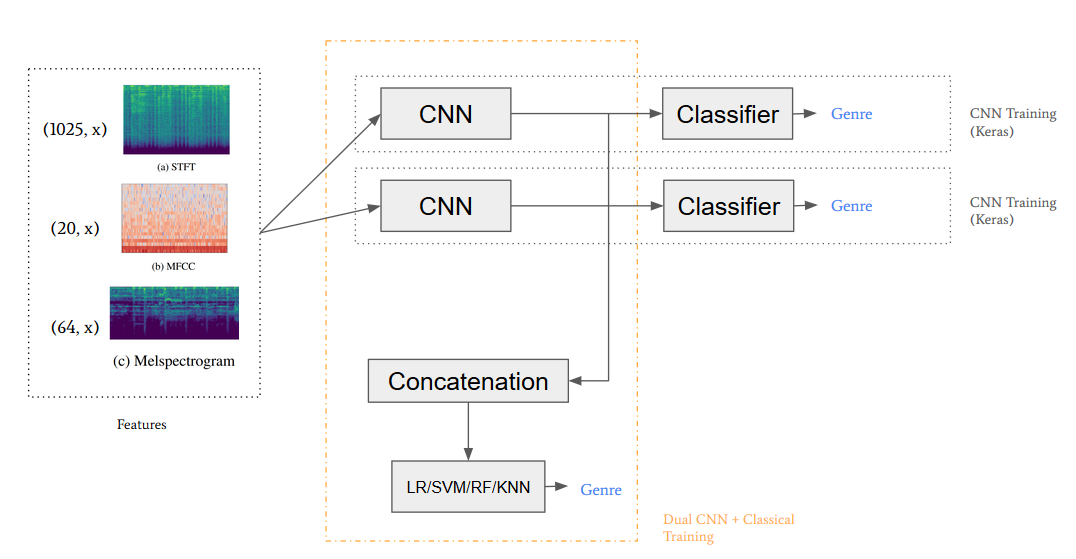
\includegraphics[width = 8cm]{DUALCNNCLASSICAL.png}}}
		\caption{Dual CNN + Classical Framework}
		\label{fig:dualcnnclassical}
	\end{figure}

	As illustrated in Figure~\ref{fig:dualcnnclassical}, the proposed Dual CNN + Classical framework consists of two inputs that is fed through two separately trained CNN models and then concatenated to a classical algorithm classifier. Two features out of STFT, MFCC, and Melspectrogram are chosen and the corresponding best model of those features are then used. The input is fed to the previously trained models and stopped right after the flatten operation. This results in two n-dimensional vectors for each of the models. Specifically for STFT, MFCC, and Melspectrogram, it would be a 1024, 256, and 512 dimensional vectors respectively. The two n-dimensional vectors would then be concatenated into a m-dimensional vector feature representation that is used for classification.
	
	The classification of the concatenated output from the two CNN models is done using a classical algorithm. The various classical algorithms used are Logistic Regression (LR), Support Vector Machine (SVM), Random Forest (RF), and K-Nearest Neighbors (KNN). All the combinations of inputs and classifier are tried to determine the best configuration of feature input and classical algorithms that results in the highest accuracy. Scikit-learn was used to implement the mentioned classifiers as well as hypertuning the parameters. The parameters that were tuned are: l2 penalty, regularization strength, and solver for LR; regularization strength and kernel for SVM; n\_estimators, criterion, and max depth for RF; n\_neighbors and metric for KNN.
	
	\section{Results} % DONE
	
	The models specified in the previous section were trained on the GTZAN and Extended Ballroom dataset and the results from the top models are shown in Table~\ref{table:resultsGTZAN} and~\ref{table:resultsExtendedBallroom}, for GTZAN and Extended Ballroom respectively. The accuracy of other published models, which are trained on the same datasets, are also included for comparison. The split of 8, which results in about 3.75 seconds of audio, was found to be the best in terms of accuracy and generalization. Thus, for the top models shown in Table ~\ref{table:resultsGTZAN} and~\ref{table:resultsExtendedBallroom}, they were trained on splits of 8. Only the proposed models used the splits of 8, while the other models, which are used for comparison, have used different sizes/lengths of input. The following sections will discuss the impact of splits, performance of the proposed models, as well as the impact of the dual inputs and using a classical algorithm as a classifier.
	
	\subsection{Impact of Splits} % DONE
	
	For the proposed simple CNN model, various splits of audio were used to determine the impact and the best split in terms of accuracy and generalization. Since the audio from both GTZAN and Extended Ballroom datasets were 30 seconds, the audio were split into 1, 2, 4, 5, 8, 10 segments. This results in at most 30 seconds input, and at the least 3 seconds input. These splits also resulted in an increase of samples, which are hugely beneficial due to only having 1,000 and about 4,000 samples for GTZAN and Extended Ballroom respectively. At a split of 8, GTZAN and Extended Ballroom will now have 10 times as much samples which results in 10,000 and about 40,000 samples respectively.
	
	The results of the models trained on different splits are shown in Table~\ref{table:splitsGTZAN} and~\ref{table:splitsExtendedBallroom} for GTZAN and Extended Ballroom respectively. In terms of GTZAN, the split clearly has a large impact on the accuracy. Specifically, for GTZAN, STFT has a large discrepancy when looking at split of 1 and 2 which has 15.5\% and 23.2\% accuracy respectively. The resulting average accuracies for each split are 80.6\%, 80.1\%, 76.0\%, 79.0\%, 52.8\%, and 49.0\% for splits 10, 8, 5, 4, 2, 1 respectively. In terms of the Extended Ballroom dataset, the resulting split accuracies are somewhat the opposite from GTZAN and more balanced and didn't have much impact. Surprisingly, a longer input resulted in higher accuracies, such as a split of 2. The resulting average accuracies for each split are 85.0\%, 86.3\%, 88.1\%, 88.4\%, 89.6\%, and 75.3\% for splits 10, 8, 5, 4, 2, 1 respectively.

	\begin{table}[!htbp] % !htbp for table positioned correctly according to text layout here
		\caption{Impact of Splits}
		\centering
		\resizebox{\columnwidth}{!}{
			\begin{tabular}[b]{ccc}
				\hline \hline
				Split & Avg Test Accuracy & Avg Train Accuracy 		\\ [0.5ex]
				\hline
				10 & 82.8\% & 89.4\%	\\
				8 & 83.2\% & 89.3\%		\\
				5 & 82.1\% & 89.5\%		\\
				4 & 83.7\% & 89.9\%		\\
				2 & 71.2\% & 80.5\%		\\
				1 & 62.2\% & 70.0\%		\\ [1ex]
				\hline \hline
		\end{tabular}}
		\label{table:splits}
	\end{table}

	In terms of GTZAN and Extended Ballroom, the best split was found to be 10 and 2 respectively when looking at accuracy. However, when not specifying the dataset and looking at the average of each split, the best resulting split was 4 with an average accuracy of 83.7\% but split of 8 was close with an accuracy of 83.2\%. The resulting average accuracies of each split are shown in Table~\ref{table:splits}. Due to a small difference, the split of 8 is the best in terms of accuracy and generalization due to the increased sample size. Training on different splits for the proposed Dual CNN + Classical model was possible but due to time constraints, it was only trained on the split of 8. The following dual input models shown in tables and discussed in the following sections will only consist of a 3.75 seconds audio input.
	
	\subsection{Performance on GTZAN} % DONE
	
	GTZAN dataset is a common benchmark in music genre classification, and thus used to compare and validate the effectiveness of the proposed models. The music genre classification accuracies of the proposed CNN and CNN+Classical models are shown in Table~\ref{table:resultsGTZAN}. Other models are also shown to compare the results of the proposed models, but keep in mind that other models used different features and lengths of input. The proposed models shown in table, which are bolded, has an input of 3.75 seconds because that length was found to be the best in terms of accuracy and generalization. 
	
	As you can see in the tables, the proposed CNN model performed relatively well compared to other models. Previous to this, the majority of the models only used STFT with some using Melspectrogram. But, with the proposed model, it is easy to see that Melspectrogram and MFCC can be used to get similar accuracies to models trained on STFT. The proposed CNN architecture using STFT, Melspectrogram, and MFCC achieved accuracies of 86.3\%, 84.0\%, and 70.1\% respectively. Compared to similar type of architectures, the 86.3\% achieved by the proposed model is close and comparable to the accuracies achieved by CNN~\cite{yang2020parallel} as shown in the table. Moreover, incorporating dual inputs and classical algorithm boosted the accuracies to be close to the top of the line models. The proposed Dual CNN + Classical models, on average, achieved about 95\%, with the highest being a Dual CNN + KNN using STFT and Melspectrogram reaching 95.8\% accuracy. Section~\ref{section:impactDual} will further discuss the impact and results of the dual inputs and classical algorithms.
	
	\begin{table}[!htbp] % !htbp for table positioned correctly according to text layout here
	\caption{Results on GTZAN}
	\centering
		\resizebox{\columnwidth}{!}{
		\begin{tabular}[b]{ccc}
			\hline \hline
			Model & Feature & Accuracy 	\\ [0.5ex]
			\hline
			MusicRecNet + SVM ~\cite{elbir2020music} & Melspectrogram & 97.6\%			\\
			\textbf{Dual CNN + KNN} & \textbf{STFT, Melspectrogram} & \textbf{95.8\%} 			\\
			\textbf{Dual CNN + KNN} & \textbf{STFT, MFCC} & \textbf{95.3\%} 			\\
			\textbf{Dual CNN + SVM} & \textbf{STFT, MFCC} & \textbf{94.0\%} 			\\
			Broadcast NN ~\cite{liu2020bottom} & Melspectrogram & 93.9\%			\\
			CNN + 1-layer RNN~\cite{yang2020parallel} & STFT & 90.2\%			\\
			CNN + 2-layer RNN~\cite{yang2020parallel} & STFT & 88.8\%			\\
			CNN~\cite{yang2020parallel} & STFT & 88.0\%							\\
			\textbf{CNN} & \textbf{STFT} & \textbf{86.3\%} 					\\
			\textbf{CNN} & \textbf{Melspectrogram} & \textbf{84.0\%} 			\\
			2-layer BRNN~\cite{schuster1997bidirectional} & STFT & 76.2\% 		\\
			\textbf{CNN} & \textbf{MFCC} & \textbf{70.1\%} 			\\[1ex]
			\hline \hline
		\end{tabular}}
	\label{table:resultsGTZAN}
	\end{table}\textsc{}

	\begin{figure}[!htpb]
		\centering
		\subfloat[\centering GTZAN STFT 8 CNN]{{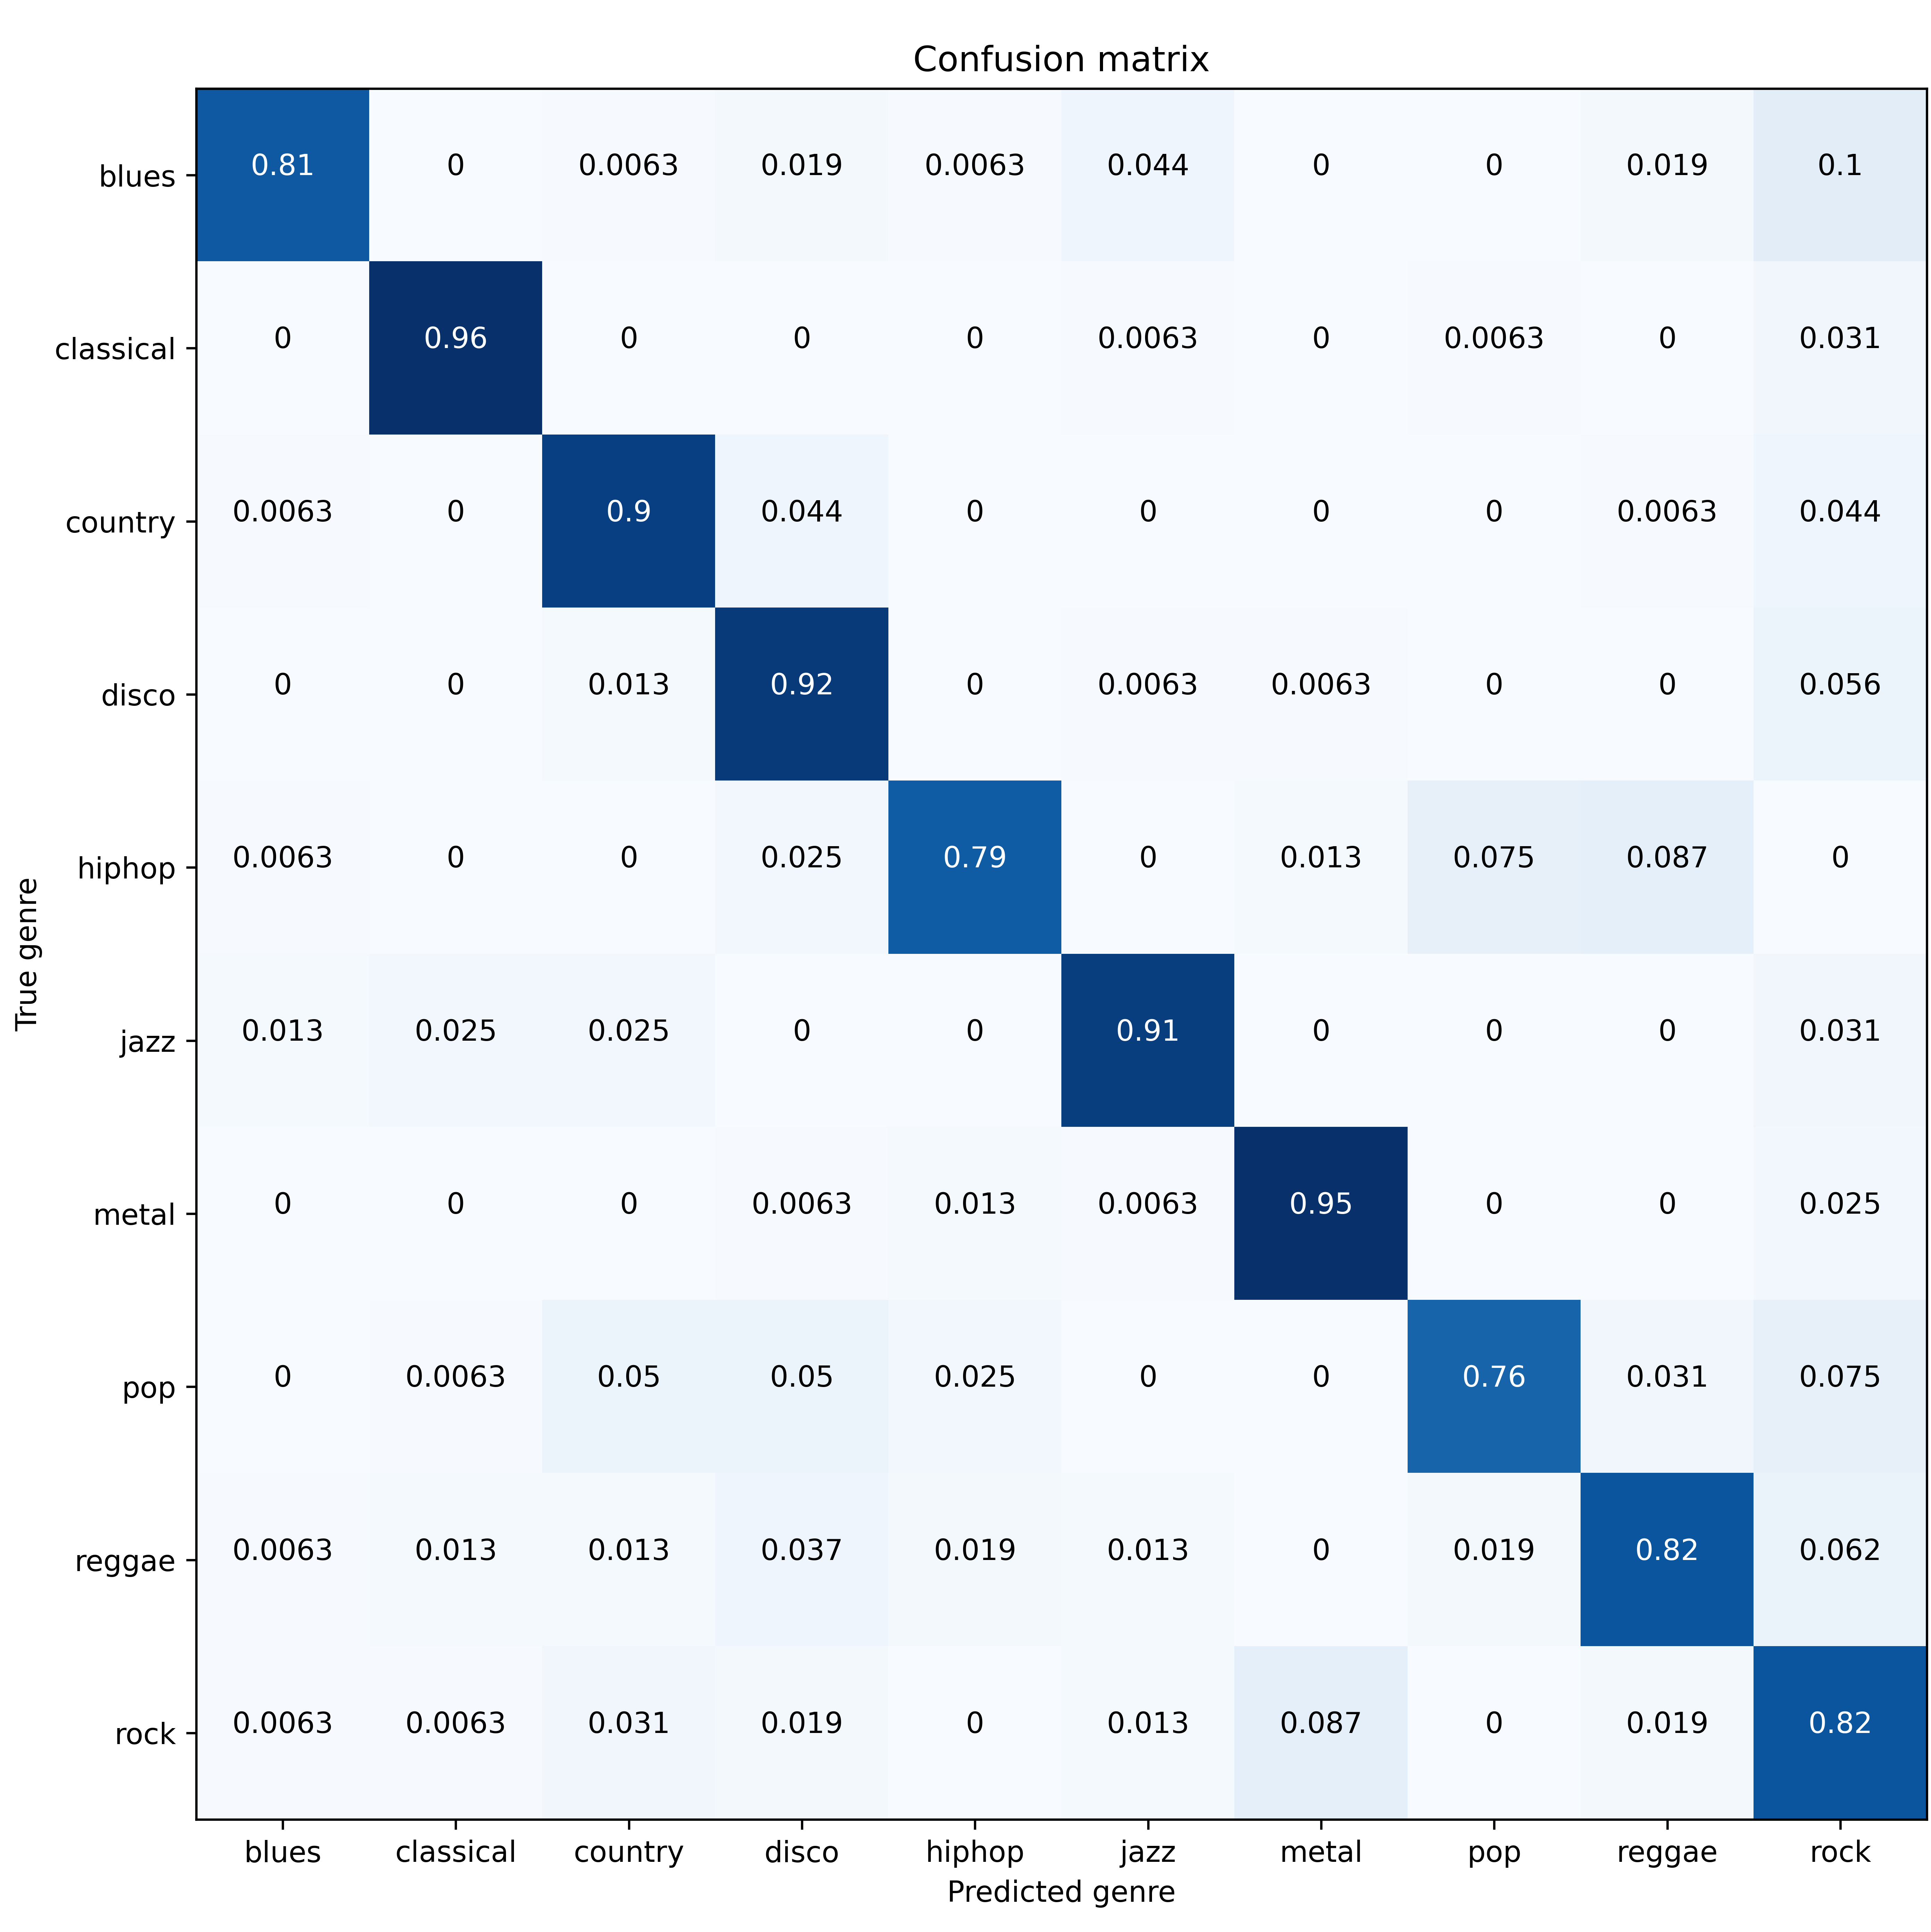
\includegraphics[width = 3.5cm]{GTZAN-STFT-8-ConfusionMatrix.png}}}
		\qquad
		\subfloat[\centering Extended Ballroom STFT 8]{{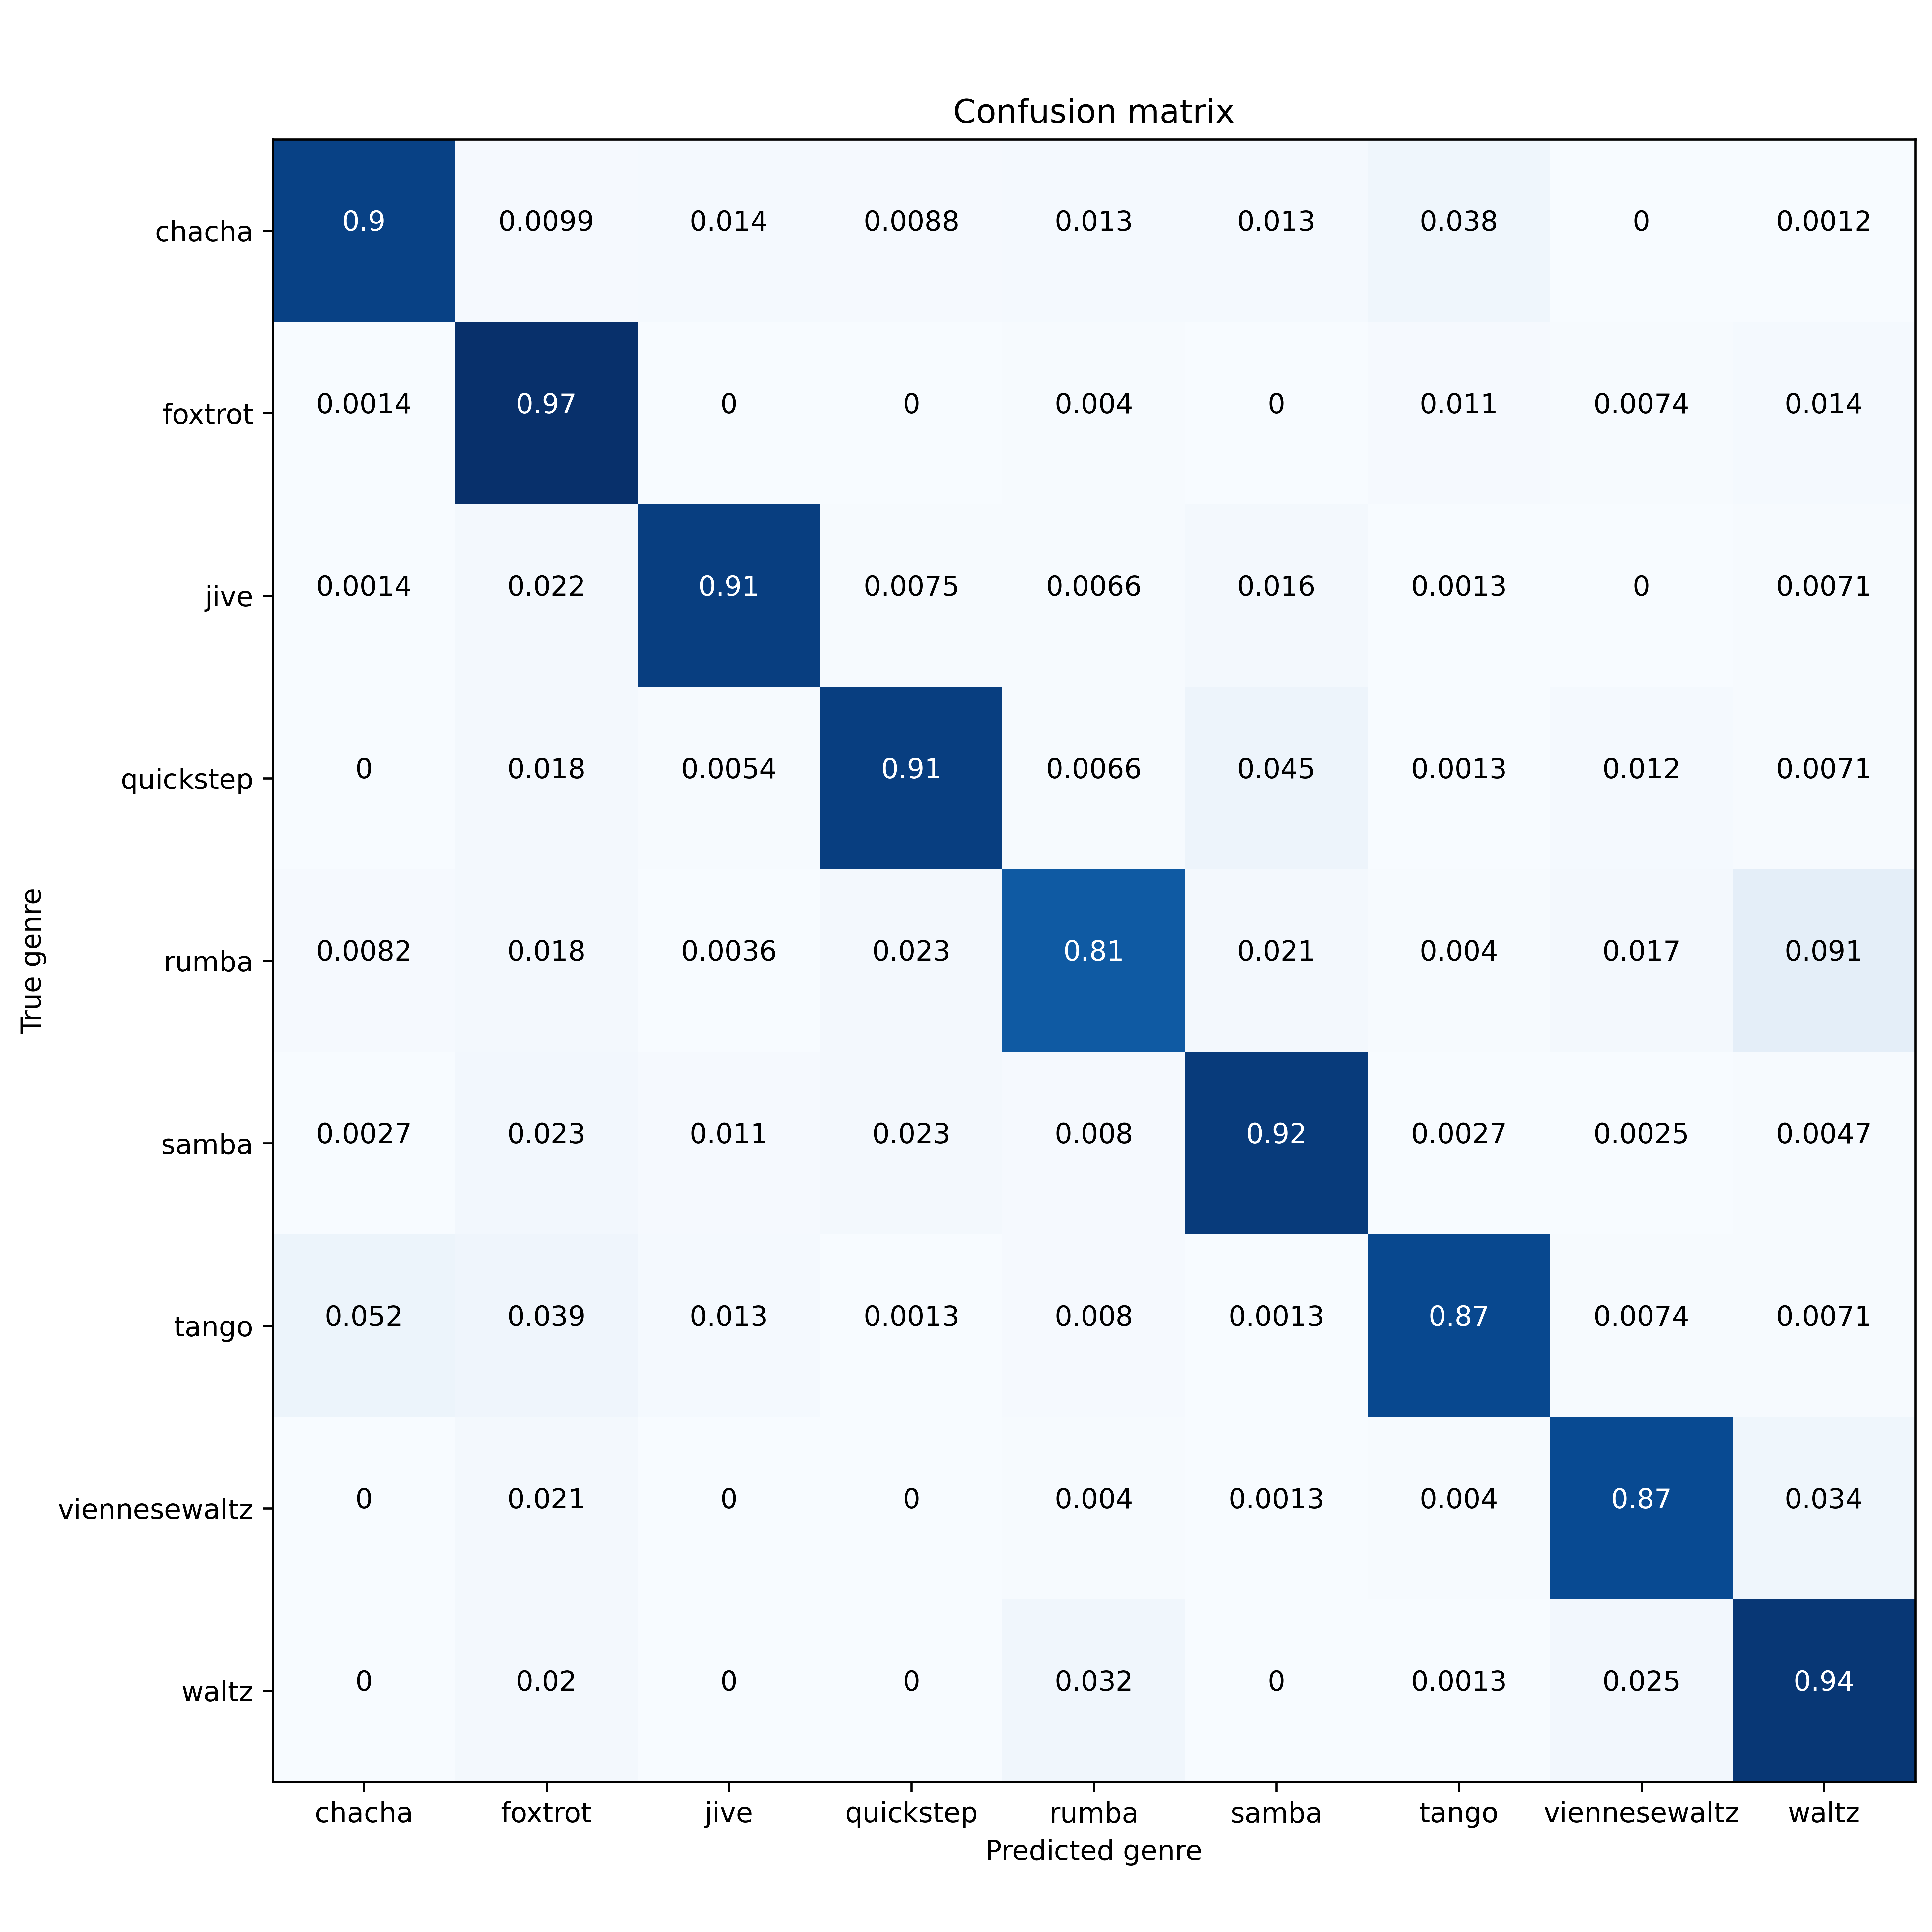
\includegraphics[width = 3.5cm]{Extended Ballroom-STFT-8-ConfusionMatrix.png}}}
		\caption{CNN Confusion Matrix}
		
		\label{fig:cnfCNN}
	\end{figure}
	
	\subsection{Performance on Extended Ballroom} % DONE
	
	Another quite common benchmark in this field is the Extended Ballroom dataset due to having about four times as much audio clips than GTZAN. Thus, the proposed models were also trained on Extended Ballroom to compare with others and further validate the effectiveness of it. As shown in Table~\ref{table:resultsExtendedBallroom}, the proposed CNN models achieved promising accuracies. Most of the other models only used STFT and the one model using Melspectrogram had the highest accuracy. With the proposed model, other features such as MFCC and Melspectrogram can be used and still have similar accuracies as models using STFT. The proposed CNN architecture using STFT, Melspectrogram, and MFCC achieved accuracies of 90.3\%, 87.0\%, and 81.5\% respectively. Compared to similar type of architectures, the 90.3\% achieved by the proposed model is close and comparable to the accuracy achieved by another CNN~\cite{yang2020parallel} as shown in the table. Moreover, incorporating dual inputs and classical algorithm boosted the accuracies to be close to the top of the line models. The proposed Dual CNN + Classical models, on average, achieved about 92\%, with the highest being a Dual CNN + SVM using STFT and MFCC reaching 92.4\% accuracy. The following section will further discuss the results and the impact of dual inputs and classical algorithms.
	
	\begin{table}[!htbp] % !htbp for table positioned correctly according to text layout here
		\caption{Results on Extended Ballroom}
		\centering
		\resizebox{\columnwidth}{!}{
		\begin{tabular}[b]{ccc}
			\hline \hline
			Model & Feature & Accuracy 	\\ [0.5ex]
			\hline
			Broadcast NN ~\cite{liu2020bottom} & Melspectrogram & 97.2\%			\\
			CNN + 2-layer RNN~\cite{yang2020parallel} & STFT & 92.5\%			\\
			\textbf{Dual CNN + SVM} & \textbf{STFT, MFCC} & \textbf{92.4\%} 			\\
			CNN + 1-layer RNN~\cite{yang2020parallel} & STFT & 92.3\%			\\
			CNN~\cite{yang2020parallel} & STFT & 92.2\%							\\
			\textbf{Dual CNN + RF} & \textbf{STFT, MFCC} & \textbf{91.9\%} 			\\
			\textbf{Dual CNN + SVM} & \textbf{STFT, Melspectrogram} & \textbf{91.9\%} 			\\
			2-layer BRNN~\cite{schuster1997bidirectional} & STFT & 90.3\% 		\\
			\textbf{CNN} & \textbf{STFT} & \textbf{90.3\%} 			\\
			\textbf{CNN} & \textbf{Melspectrogram} & \textbf{87.0\%} 	\\
			\textbf{CNN} & \textbf{MFCC} & \textbf{81.5\%} 			\\[1ex]
			\hline \hline
		\end{tabular}}
	\label{table:resultsExtendedBallroom}
	\end{table}

	\begin{figure}[!htpb]
		\centering
		\subfloat[\centering GTZAN STFT+MELSPECTROGRAM 8 CNN+KNN]{
			{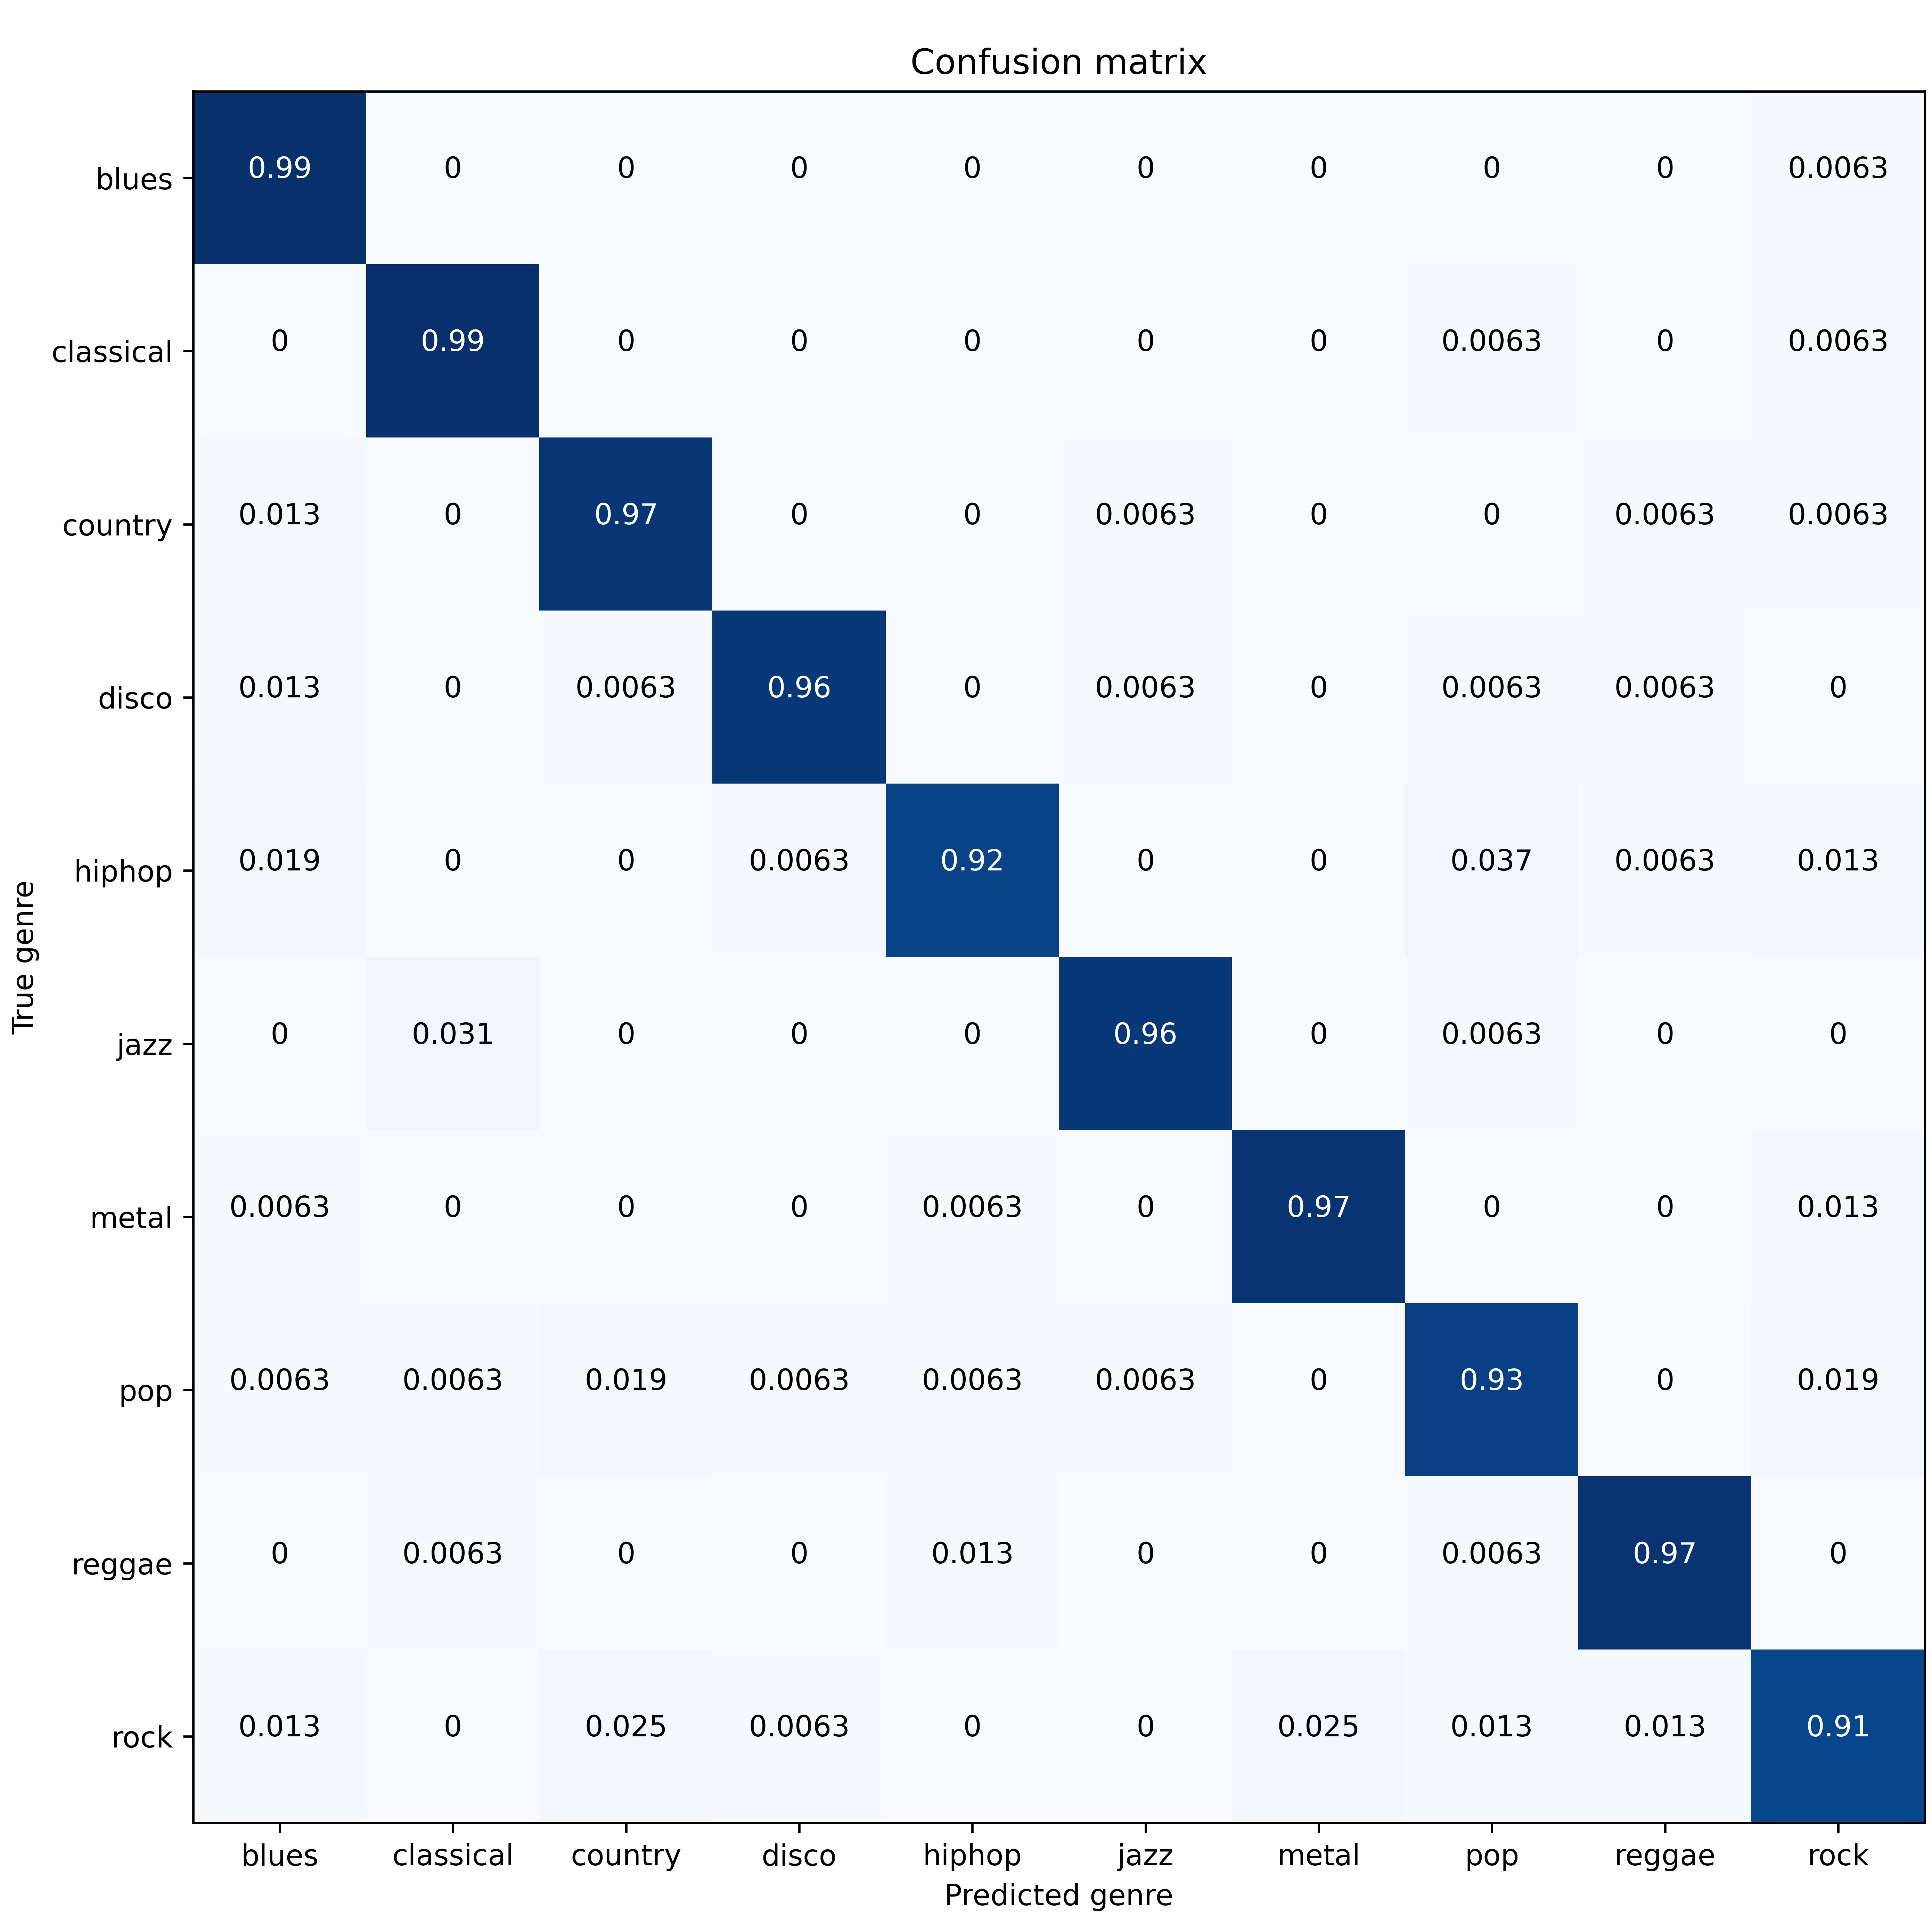
\includegraphics[width = 3.5cm]{7628_CNN_STFT_MELSPECTROGRAM_KNN_GTZAN_8-ConfusionMatrix.png}}}
		\qquad
		\subfloat[\centering Extended Ballroom STFT+MFCC 8 CNN+SVM]{
			{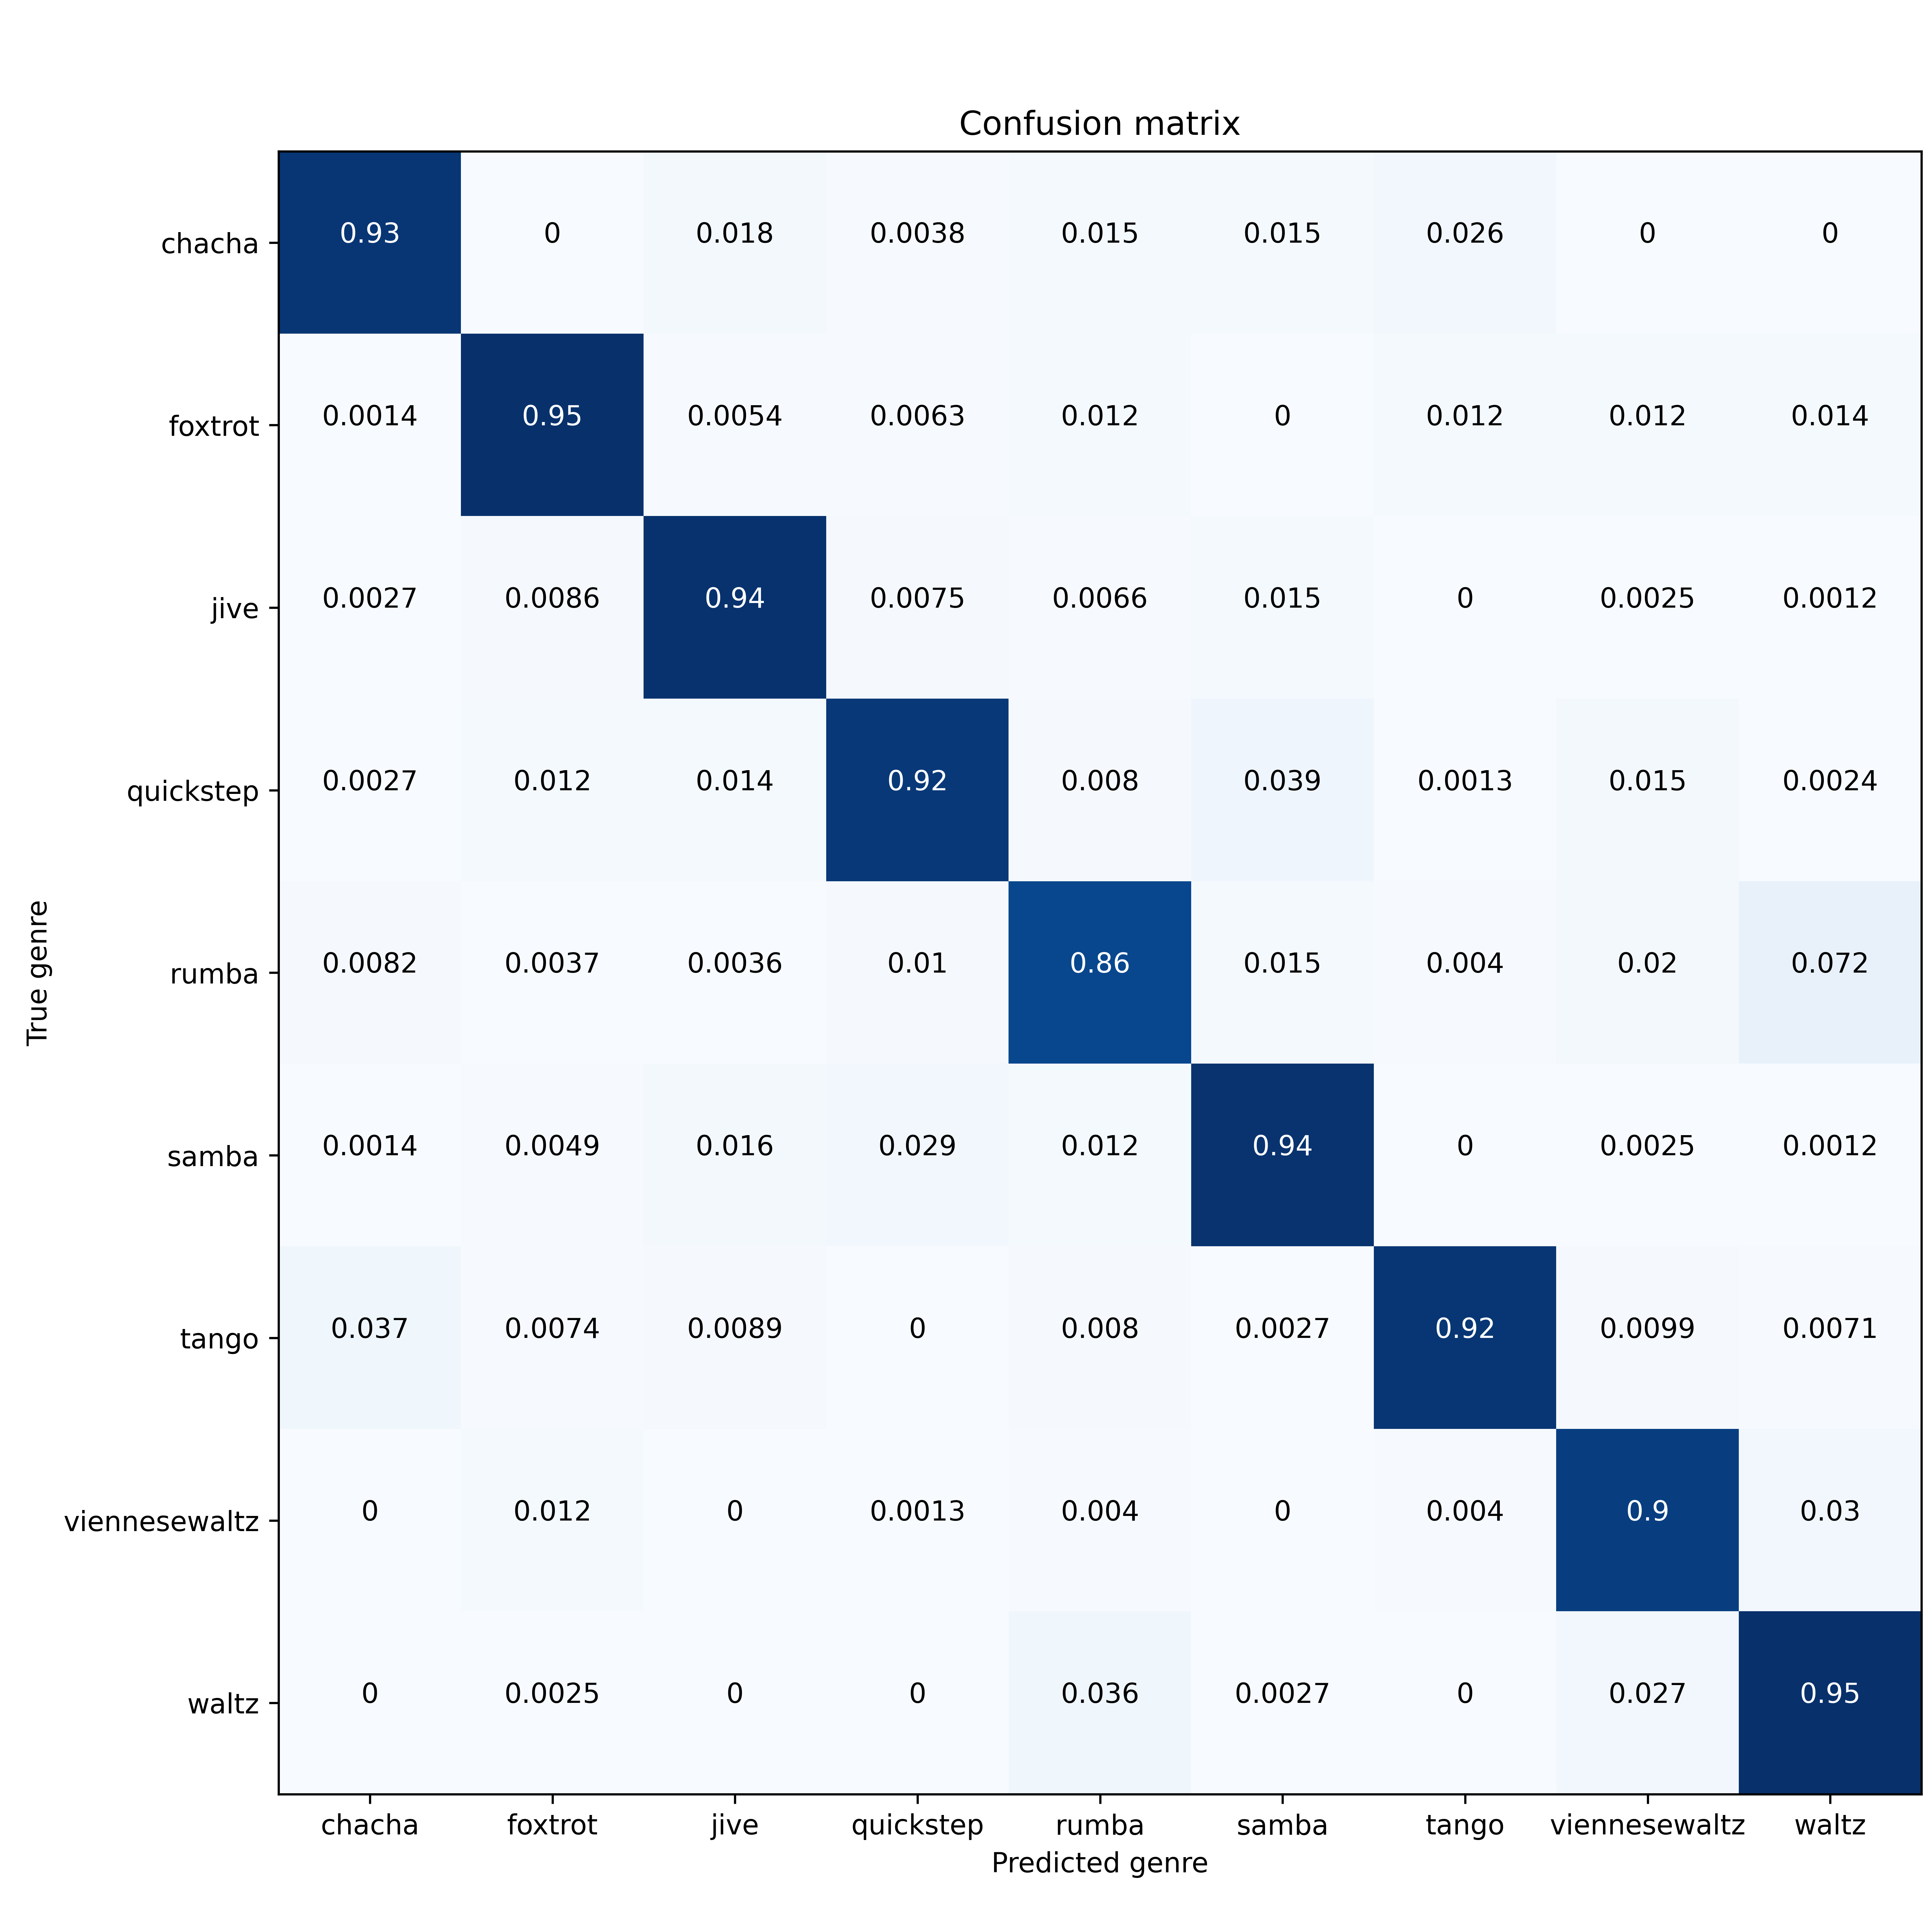
\includegraphics[width = 3.5cm]{757_CNN_STFT_MFCC_SVM_EXTENDEDBALLROOM_8-ConfusionMatrix.png}}}
		\caption{CNN+Classical Confusion Matrix}
		
		\label{fig:cnfCNNClassical}
	\end{figure}
	
	\subsection{Impact of Dual Inputs and Classical Algorithms} % DONE
	\label{section:impactDual}
	
	In terms of GTZAN, with the proposed Dual CNN + Classical architecture, the accuracies were boosted by 8 to 15 percent. All the models benefited from having an additional input as well as having used a classical algorithm as a classifier. A CNN model using STFT, and MFCC only achieved an accuracy of 86.3\% and 70.1\% respectively. However when STFT and MFCC are combined and KNN was used as a classifier, the resulting accuracy is 95.3\% which clearly shows that there is a huge benefit to having multiple feature inputs. This can be seen clearly on Figures~\ref{fig:cnfCNN} and~\ref{fig:cnfCNNClassical} with the moderately accurate genres of the CNN model becoming highly accurate when dual inputs and a classical algorithm is used. The proposed top model trained on GTZAN dataset is a Dual CNN + KNN model using STFT and Melspectrogram feature inputs which achieved 95.8\% accuracy, only 1.8\% lower than the top of the line model. The results in Table~\ref{table:resultsGTZAN} demonstrate that dual feature inputs and use of classical algorithms as a classifier can significantly improve the performance of models that are not using a classical algorithm classifier and only one feature input.
	
	In terms of Extended Ballroom, the increase in accuracies aren't that high but still significant, boosting the accuracies by 2 to 9 percent. Also, as shown in Figures~\ref{fig:cnfCNN} and~\ref{fig:cnfCNNClassical}, the addition of features significantly increased the accuracy of the model in terms of the rumba, tango, and viennesewaltz genre. All the models benefited, albeit only a little compared to models trained in GTZAN, from having an additional input as well using a classical algorithm as a classifier. As shown in Table~\ref{table:resultsExtendedBallroom}, STFT plays a huge part in reaching high accuracies due to all the dual input models using STFT. Looking at the CNN model with only a STFT input reaching 90.3\% accuracy, the addition of other features only boosted the accuracy by about 2\%. However, this small increase in accuracy is still significant due to lots of other models also having the same accuracies. Most of the models shown are around 92\% and the best proposed model achieved 92.4\% with a Dual CNN + SVM with STFT and MFCC feature input.

	Tables~\ref{table:dualCNN+classicalGTZAN} and~\ref{table:dualCNN+classicalExtendedBallroom} presents a more comprehensive table with all the possible dual input and classical model with the resulting accuracy. Looking at each of the models, STFT clearly has the highest impact on the accuracy, with the top models including STFT as one of two feature inputs. The addition of a classical algorithm as a classifier also significantly boosted the accuracies of the models. Overall, all the models, whether it be trained on GTZAN and Extended Ballroom, benefited from having an additional input as well as using a classical algorithm as a classifier. 
	
	\begin{table}[!htbp] % !htbp for table positioned correctly according to text layout here
		\caption{Impacts of Dual Inputs + Classical Algorithm in GTZAN}
		\centering
		\resizebox{\columnwidth}{!}{
			\begin{tabular}[b]{ccc}
				\hline \hline
				Model & Feature & Accuracy 		\\ [0.5ex]
				\hline
				Dual CNN + KNN & STFT, MELSPECTROGRAM & 95.8\%				\\
				Dual CNN + KNN & STFT, MFCC & 95.3\%				\\
				Dual CNN + SVM & STFT, MELSPECTROGRAM & 95.0\%				\\
				Dual CNN + SVM & STFT, MFCC & 94.0\%				\\
				Dual CNN + LR & STFT, MELSPECTROGRAM & 93.2\%				\\
				Dual CNN + LR & STFT, MFCC & 92.1\%				\\
				Dual CNN + RF & STFT, MFCC & 91.6\%				\\
				Dual CNN + RF & STFT, MELSPECTROGRAM & 91.6\%				\\
				Dual CNN & STFT, MFCC & 90.8\%				\\
				Dual CNN & STFT, MELSPECTROGRAM & 90.5\%				\\
				Dual CNN + KNN & MFCC, MELSPECTROGRAM & 89.7\%				\\
				Dual CNN & MFCC, MELSPECTROGRAM & 89.1\%				\\
				Dual CNN + SVM & MFCC, MELSPECTROGRAM & 89.1\%				\\
				Dual CNN + LR & MFCC, MELSPECTROGRAM & 86.9\%				\\
				Dual CNN + RF & MFCC, MELSPECTROGRAM & 85.3\%				\\ [1ex]
				\hline \hline
		\end{tabular}}
		\label{table:dualCNN+classicalGTZAN}
	\end{table}
	
	\begin{table}[!htbp] % !htbp for table positioned correctly according to text layout here
		\caption{Impacts of Dual Inputs + Classical Algorithm in Extended Ballroom}
		\centering
		\resizebox{\columnwidth}{!}{
			\begin{tabular}[b]{ccc}
				\hline \hline
				Model & Feature & Accuracy 		\\ [0.5ex]
				\hline
				Dual CNN + SVM & STFT, MFCC & 92.4\%				\\
				Dual CNN + RF & STFT, MFCC & 91.9\%				\\
				Dual CNN + SVM & STFT, MELSPECTROGRAM & 91.9\%				\\
				Dual CNN + KNN & STFT, MFCC & 91.8\%				\\
				Dual CNN + RF & STFT, MELSPECTROGRAM & 91.5\%				\\
				Dual CNN + LR & STFT, MFCC & 91.4\%				\\
				Dual CNN + KNN & STFT, MELSPECTROGRAM & 91.4\%				\\
				Dual CNN & STFT, MFCC & 91.3\%				\\
				Dual CNN + LR & STFT, MELSPECTROGRAM & 91.2\%				\\
				Dual CNN & STFT, MELSPECTROGRAM & 91.1\%				\\
				Dual CNN + SVM & MFCC, MELSPECTROGRAM & 89.8\%				\\
				Dual CNN & MFCC, MELSPECTROGRAM & 89.1\%				\\
				Dual CNN + LR & MFCC, MELSPECTROGRAM & 88.9\%				\\
				Dual CNN + RF & MFCC, MELSPECTROGRAM & 88.3\%				\\
				Dual CNN + KNN & MFCC, MELSPECTROGRAM & 87.7\%				\\ [1ex]
				\hline \hline
		\end{tabular}}
		\label{table:dualCNN+classicalExtendedBallroom}
	\end{table}
	
	\section{Conclusion} % DONE
	
	In conclusion, as shown in Tables~\ref{table:resultsGTZAN} and~\ref{table:resultsExtendedBallroom}, adding an additional feature input along with using a classical algorithm as a classifier resulted in high accuracies that are close to the top of the line models in this field. The proposed Dual CNN + Classical framework outperforms the base CNN model, achieving around 95.8\% and 92.4\% compared to 86.3\% and 90.3\% accuracy on GTZAN and Extended Ballroom respectively. While STFT is a huge reason of the high accuracy, the addition of other feature inputs still have a significant impact on accuracy considering the top models are in the range of 90\% accuracy. Most of the top of the line models previous to this have only used one spectrogram as an input. However, as shown in this paper, various single feature input models by other people could likely be improved by adding more feature inputs and utilizing a classical algorithm for a classifier. Thus, there are still improvements to be made by the top models in music genre classification, and utilizing multiple different feature inputs such as spectrograms may be the most significant.
	
	\section{Future Work} % DONE
	
	Considering that I used two feature inputs rather than the usual of one, in the future I may try to add more inputs. Adding more inputs will result in diminishing returns but at such a high level accuracy, a tiny increase is still significant. More research would also probably result in more effective spectrograms or representations of music that I can utilize. More data is definitely beneficial as even the segmented audio clips of GTZAN and Extended Ballroom, which at max was 10,000 and 40,000 samples, resulted in the models overfitting. In terms of data, I could use Free Music Archive (FMA) and the Million Song Dataset which consists of 0.1 million and 1 million songs respectively. Also, I could have utilized a Recurrent Neural Network (RNN) in combination with CNNs as Yang et al.~\cite{yang2020parallel} has shown that CNNs with a parallel RNN block achieves better performance than CNNs alone. I simply didn't have enough time to further include RNN in combination with CNN, classical algorithms, and additional feature inputs. In the future, there are many different ways I can do to further improve my models.
		
	{\small
		\bibliographystyle{ieee_fullname}
		\bibliography{egbib}
	}

	% These tables of STFT, gram, MFCC splits should be after conclusion. Cuz lots of data, not really essential, just the best one. Also the confusoin matrix cuz of the amount of psace it takes up

	\begin{table}[!htbp] % !htbp for table positioned correctly according to text layout here
		\caption{Impact of Splits in GTZAN}
		\centering
		\resizebox{\columnwidth}{!}{
			\begin{tabular}[b]{cccc}
				\hline \hline
				Model & Feature & Split & Accuracy 		\\ [0.5ex]
				\hline
				CNN & STFT &  10 & 82.5\%				\\
				CNN & STFT &  8 & 86.3\%				\\
				CNN & STFT &  5 & 85.5\%				\\
				CNN & STFT &  4 & 86.3\%				\\
				CNN & STFT &  2 & 23.2\%				\\
				CNN & STFT &  1 & 15.5\%				\\
				CNN & MFCC &  10 & 75.9\%				\\
				CNN & MFCC &  8 & 70.1\%				\\
				CNN & MFCC &  5 & 61.5\%				\\
				CNN & MFCC &  4 & 67.0\%				\\
				CNN & MFCC &  2 & 61.5\%				\\
				CNN & MFCC &  1 & 60.0\%				\\
				CNN & Melspectrogram & 10 & 83.3\% 		\\
				CNN & Melspectrogram & 8 & 84.0\% 		\\
				CNN & Melspectrogram & 5 & 81.5\% 		\\
				CNN & Melspectrogram & 4 & 83.7\% 		\\
				CNN & Melspectrogram & 2 & 73.7\% 		\\
				CNN & Melspectrogram & 1 & 71.5\% 		\\ [1ex]
				\hline \hline
		\end{tabular}}
		\label{table:splitsGTZAN}
	\end{table}
	
	\begin{table}[!htbp] % !htbp for table positioned correctly according to text layout here
		\caption{Impact of Splits in Extended Ballroom}
		\centering
		\resizebox{\columnwidth}{!}{
			\begin{tabular}[b]{cccc}
				\hline \hline
				Model & Feature & Split & Accuracy 		\\ [0.5ex]
				\hline
				CNN & STFT &  10 & 89.4\%				\\
				CNN & STFT &  8 & 90.3\%				\\
				CNN & STFT &  5 & 92.6\%				\\
				CNN & STFT &  4 & 90.3\%				\\
				CNN & STFT &  2 & 92.1\%				\\
				CNN & STFT &  1 & 92.6\%				\\
				CNN & MFCC &  10 & 80.5\%				\\
				CNN & MFCC &  8 & 81.5\%				\\
				CNN & MFCC &  5 & 84.5\%				\\
				CNN & MFCC &  4 & 83.4\%				\\
				CNN & MFCC &  2 & 85.6\%				\\
				CNN & MFCC &  1 & 41.8\%				\\
				CNN & Melspectrogram & 10 & 85.0\% 		\\
				CNN & Melspectrogram & 8 & 87.0\% 		\\
				CNN & Melspectrogram & 5 & 89.4\% 		\\
				CNN & Melspectrogram & 4 & 90.4\% 		\\
				CNN & Melspectrogram & 2 & 91.1\% 		\\
				CNN & Melspectrogram & 1 & 91.4\% 		\\ [1ex]
				\hline \hline
		\end{tabular}}
		\label{table:splitsExtendedBallroom}
	\end{table}
	
\end{document}